%%%%%%%%%%%%%%%%%%%%%%%%%%%%%%%%%%%%%%%%%
% a0poster Landscape Poster
% LaTeX Template
% Version 1.0 (22/06/13)
%
% The a0poster class was created by:
% Gerlinde Kettl and Matthias Weiser (tex@kettl.de)
% 
% This template has been downloaded from:
% http://www.LaTeXTemplates.com
%
% License:
% CC BY-NC-SA 3.0 (http://creativecommons.org/licenses/by-nc-sa/3.0/)
%
%%%%%%%%%%%%%%%%%%%%%%%%%%%%%%%%%%%%%%%%%

%----------------------------------------------------------------------------------------
%	PACKAGES AND OTHER DOCUMENT CONFIGURATIONS
%----------------------------------------------------------------------------------------

\documentclass[a0,landscape]{a0poster}

\setlength{\topmargin}{-2cm}

\usepackage{multicol} % This is so we can have multiple columns of text side-by-side 
\columnsep=90pt % This is the amount of white space between the columns in the poster 
\columnseprule=0pt % This is the thickness of the black line between the columns in the poster

\usepackage[svgnames]{xcolor} % Specify colors by their 'svgnames',
                              % for a full list of all colors
                              % available see here: http://www.latextemplates.com/svgnames-colors

\usepackage{times} % Use the times font
%\usepackage{palatino} % Uncomment to use the Palatino font

\usepackage{graphicx} % Required for including images
\graphicspath{{figures/}} % Location of the graphics files
\usepackage{booktabs} % Top and bottom rules for table
\usepackage[font=small,labelfont=bf]{caption} % Required for specifying captions to tables and figures 
 \usepackage{amsfonts,
  amsmath, amsthm, amssymb} % For math fonts, symbols and environments
\usepackage{wrapfig} % Allows wrapping text around tables and figures

\usepackage{Sweave}
\begin{document}
\Sconcordance{concordance:lau_esa2015.tex:/Users/hermes/projects/esa2015/poster_2015/docs/poster/lau_esa2015.Rnw:%
1 43 1 1 0 203 1 1 31 1 3 17 1 1 49 1 3 59 1}


%----------------------------------------------------------------------------------------
%	POSTER HEADER 
%----------------------------------------------------------------------------------------

% The header is divided into three boxes:
% The first is 55% wide and houses the title, subtitle, names and university/organization
% The second is 25% wide and houses contact information
% The third is 19% wide and houses a logo for your university/organization or a photo of you
% The widths of these boxes can be easily edited to accommodate your content as you see fit

\begin{minipage}[b]{0.65\linewidth}
\veryHuge \color{Red} \textbf{Temporal scales of coupled ecosystem
  processes provide a benchmark for alternate ecosystem states}
\color{Black}\\ % Title 
\Huge\textit{Photosynthesis and decomposition in a model micro-ecosystem}\\[1cm] % Subtitle 
\huge \textbf{Matthew K. Lau \& Aaron M. Ellison}\\ % Author(s) 
\huge Harvard Forest, Harvard University \\ % University/organization
\end{minipage}
%
\begin{minipage}[b]{0.20\linewidth}
\color{DarkSlateGray}\Large \textbf{Contact Information:}\\ 
Harvard Forest\\ % Address 
Harvard University\\ 324 N Main St, Petersham, MA, USA\\ 
Phone: +1 (978) 756-6165\\ % Phone number 
Email: \texttt{matthewklau@fas.harvard.edu}\\ % Email address
\end{minipage}
%
\begin{minipage}[t]{0.12\linewidth}

\includegraphics[width=17cm]{hf.pdf} % Logo or a photo of you, adjust its dimensions here
%% 
\includegraphics[width=10cm]{harvard.png} % Logo or a photo of you, adjust its dimensions here
\end{minipage}

\vspace{3cm} % A bit of extra whitespace between the header and poster
             % content

%----------------------------------------------------------------------------------------

\begin{multicols}{3} % This is how many columns your poster will be broken into, a poster with many figures may benefit from less columns whereas a text-heavy poster benefits from more

%----------------------------------------------------------------------------------------
%	ABSTRACT
%----------------------------------------------------------------------------------------

\color{DarkBlue} % Navy color for the abstract

\section*{Background and Overview}
  
  \begin{itemize}
  \item Ecosystem dynamics can lead to sudden, recalcitrant state changes,
  \item Here, we further develop and apply an ecosystem model based on
    the food web of the carnivorous plant, \textit{Sarracenia
      purpurea}, to simulate oxygen production and explore the impact
    of simultaneously altering key parameters,
  \item We found three main results:
    \begin{enumerate}
    \item The micro-ecosystem model reproduced key behaviors of
      the real pitcher plant food web
    \item Sensitivity analysis revealed parameter combinations that
      produce alternative ecosystem states
    \item Differences in photosynthesis and decomposition rates lead
      to both alternative states and hysteresis,
    \end{enumerate}
  \item These results support previous findings that the timing of
    processes can lead to shifts in ecosystem state. 
  \end{itemize}

%----------------------------------------------------------------------------------------
%	INTRODUCTION
%----------------------------------------------------------------------------------------

% \color{SaddleBrown} % SaddleBrown color for the introduction

%% \section*{Background}

%% \begin{itemize}
%% \item Stability
%% \item Alternative states
%% \item Tipping points
%% \item The pitcher plant micro-ecosystem
%% \item Hastings, temporal scales paper
%% \end{itemize}

%----------------------------------------------------------------------------------------
%	OBJECTIVES
%----------------------------------------------------------------------------------------

\color{DarkSlateGray} % DarkSlateGray color for the rest of the content

%% \section*{Hypotheses}


%----------------------------------------------------------------------------------------
%	MATERIALS AND METHODS
%----------------------------------------------------------------------------------------

\section*{Methods}

%------------------------------------------------

\begin{center}
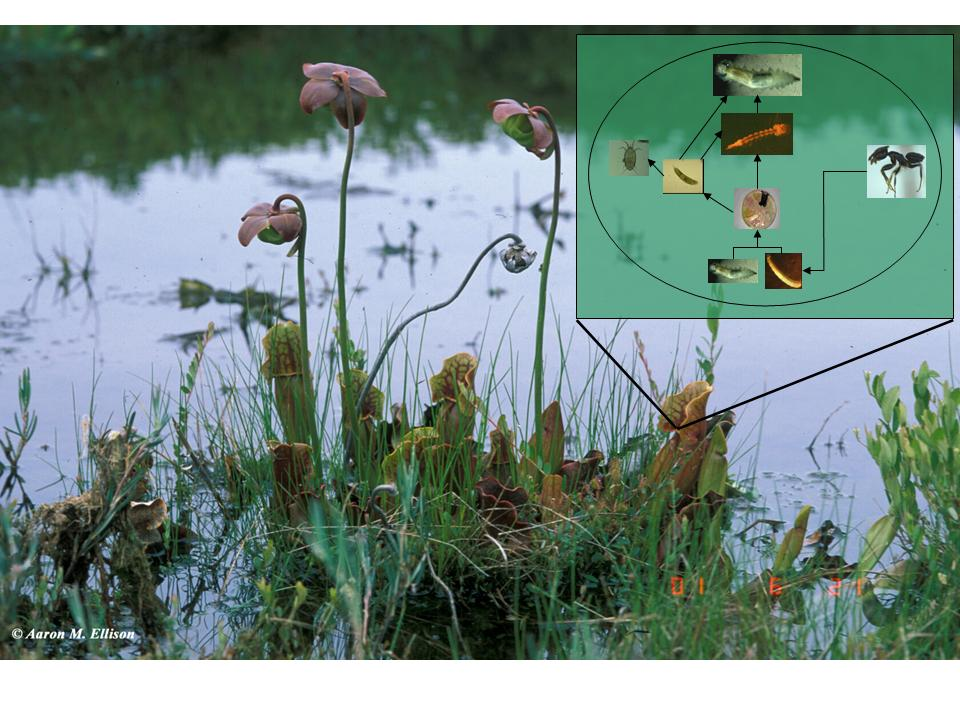
\includegraphics[width=0.75\linewidth]{spfoodweb}
\captionof{figure}{Pitcher plant and food web.}
\end{center}

\subsection*{Pitcher Plant Micro-Ecosystem Model}

A general model that produces alternative ecosystem states can be
represented as: $\frac{dx}{dt} = a - bx + r f(x)$. Where, $x$ =
observed variable, $a$ = positively correlated state variable, $b$ =
negatively correlated state variable, $rf(x)$ = positive feedback
loop, where $r$ controls the rate and $f(x)$ determines the shape of
the state transition.

%% R^2 = $ 0.1092

\begin{center}\vspace{1cm}
\begin{tabular}{l l}
\toprule
\textbf{Component} & Equation \\
\midrule
Oxygen & $x_{t+1} = a_t A_t - \left\{m + a_t \frac{w+t}{K + w_t}\right\} + D_t(x_t)$ \\
Photosynthesis & $  A = A_{max} \left\{ 1 - e^{-0.3 (PAR - LCP)} \right\} $\\
PAR & $PAR = c \sin(2 \pi f)$\\
Decomposition & $w_t = e^{-\beta w_0 t}$\\
Oxygenation & $a_t+1 = a_t \left\{ \frac{a'_{max}-a'_{min}}{1+e^{-s n_t - d}} + a'_{min}\right\}$ \\
Nutrient Release & $n_t = \frac{w_t x_t}{c}$ \\
\bottomrule
\end{tabular}
\captionof{table}{The \textit{S. purpurea} micro-ecosystem model.}
\end{center}\vspace{1cm}

\subsection*{Sensitivity Analysis Simulations}

Because the micro-ecosystem model is a coupled, non-linear dynamic
equation, we conducted simulations in which we varied three key
parameters in the model: $w$ the prey mass added, $\beta$ the
decomposition rate and $d$ the inflection point of the nutrient
augmentation function. 

%----------------------------------------------------------------------------------------
%	RESULTS 
%----------------------------------------------------------------------------------------

\section*{Results}

\begin{block}{}
\setkeys{Gin}{width=0.65\linewidth}
\begin{center}

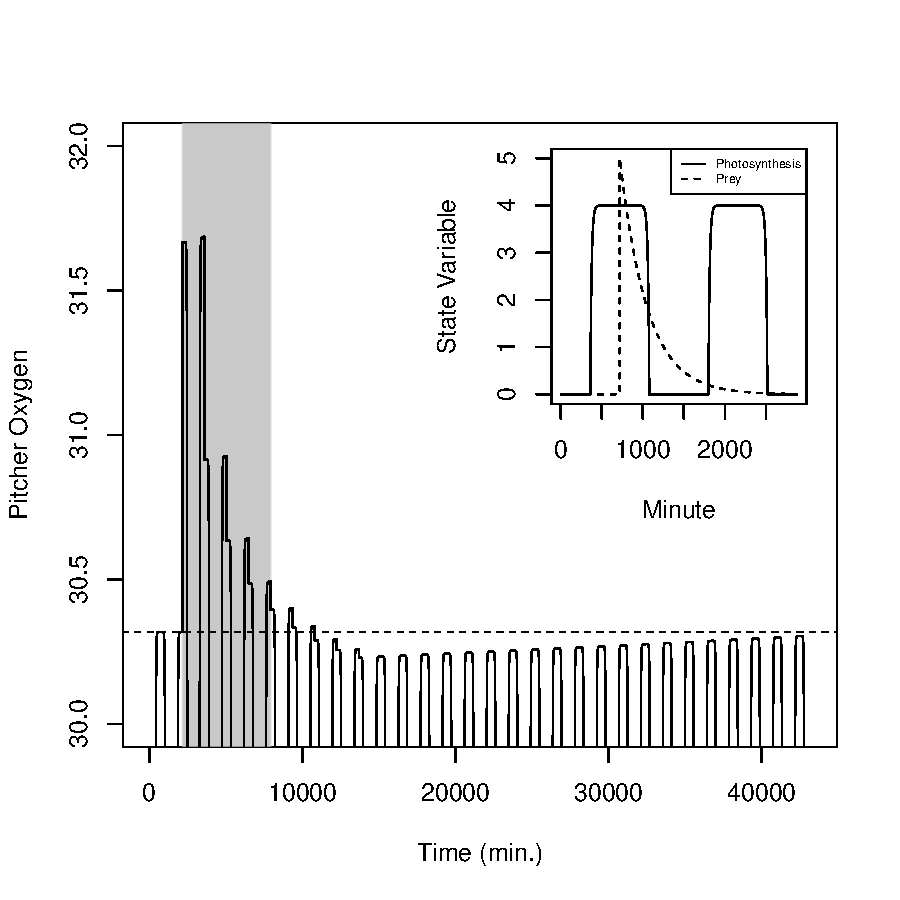
\includegraphics{lau_esa2015-base}

\captionof{figure}{The pitcher plant micro-ecosystem model exhibited several
behaviors similar to those of real \textit{S. purpurea} pitcher
plants, including: diurnal cycling of O$_2$ and 48 hours to complete
decomposition of prey (inset plot), altered O$_2$ production with prey
addition (grey region), hysteresis occurs when prey addition stops
(time = 9360 min).}
 
\end{center}

\end{block}



\begin{block}
\setkeys{Gin}{width=0.65\linewidth}  
\begin{center}
  
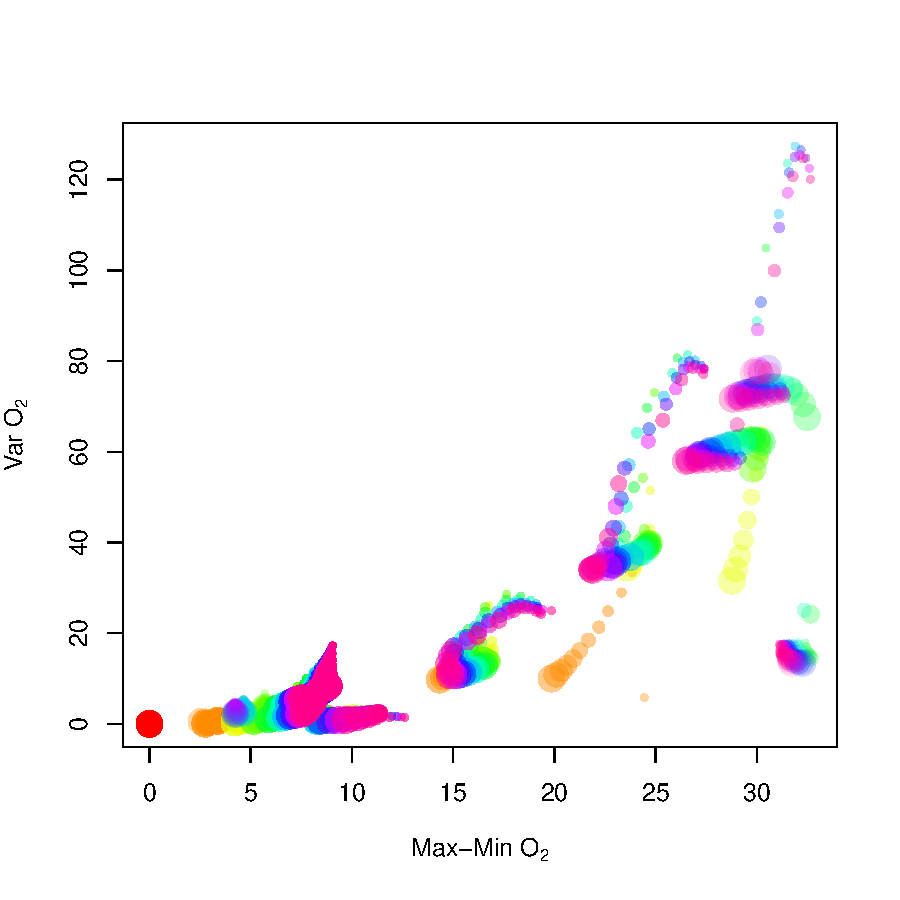
\includegraphics{lau_esa2015-sens}

\captionof{figure}{The variance and range of the O$_2$ dynamics were
  affected by prey mass (\textit{w}) added (color: red = 0 to blue=10), the decomposition rate ($\beta$) (size: smallest = 0.001 to largest = 0.011) and the inflection point (\textit{d}) of O$_2$ augmentation (opacity: lightest = -5 to darkest = 5).}

\end{center}
\end{block}

%----------------------------------------------------------------------------------------
%	CONCLUSIONS
%----------------------------------------------------------------------------------------

\color{SaddleBrown} % SaddleBrown color for the conclusions to make them stand out

\section*{Conclusions}

\begin{itemize}
\item Exploration of the parameter space for the model supports the
  presence of alternative states and the potential for tipping points
  resulting from the impact of the rate of decomposition and
  photosynthesitic augmentation.
\item These results suggest that identifying the flow of important
  components (e.g., nutrients) among compartments in ecosystems and
  using snap-shot data to compare the temporal scale of these flow
  rates can help to detect systems prone to critical transitions.
\item We are currently developing a toolbox for exploring ecosystems
  models using a web-based dynamic modeling framework available at:
  https://github.com/HarvardForest/ecoapps.
\end{itemize}

\color{DarkSlateGray} % Set the color back to DarkSlateGray for the rest of the content

%----------------------------------------------------------------------------------------
%	FORTHCOMING RESEARCH
%----------------------------------------------------------------------------------------

%% \section*{Forthcoming}


%----------------------------------------------------------------------------------------
%	REFERENCES
%----------------------------------------------------------------------------------------

%% \nocite{*} % Print all references regardless of whether they were cited in the poster or not
%% \bibliographystyle{plain} % Plain referencing style
%% \bibliography{sample} % Use the example bibliography file sample.bib

%----------------------------------------------------------------------------------------
%	ACKNOWLEDGEMENTS
%----------------------------------------------------------------------------------------

\section*{Acknowledgements}

Thanks are owed to a number of collaborators, including B. Baiser
(UFL), N. Gotelli (UVM) and A. Northrop (UVM). Funding was provided by
NSF Grant DEB 11-44056. 

%----------------------------------------------------------------------------------------

\vspace{-2cm}

\end{multicols}
\end{document}
